\chapter{Versuchsdurchführung}
\section{Tieftemperatur Supraleitung}
Im ersten Versuchsteil sollten wir das Verhalten eines Niob-Films und eines Spulenkörpers mit Bleikern bei sehr niedrigen Temperaturen in Abhängigkeit eines Magnetfelds beobachten. Dazu wurde ein vorgefertigter Messaufbau, der an einem Edelstahlstab befestigt war in eine mit flüssigem Helium gefüllte Kanne  gesenkt (siehe Abb. \ref{tieftemp_aufbau}) und somit langsam auf ca. 4,5K abgekühlt. Nach Erreichen des thermodynamischen Gleichgewichts zwischen Helium und Probenaufbau wurde mit der Messung des Spulenkörpers begonnen: Dazu wurde die Temperatur mittels einer im Probenkörper verbauten Heizspule langsam schrittweise von 4,45K auf 8,03K erhöht und jeweils das Magnetfeld um den Probenkörper durchgesweept. Dies erfolgte über die supraleitende Magnetspule, die sich in der Hülle des Probenkörpers befand (siehe Abb. \ref{tieftemp_aufbau}). Die Ansteuerung der Magnetspule, sowie die Messung des Spannungsabfalls am Probenkörper erfolgten hierbei automatisch über ein Computerprogramm. 


\begin{figure}[H]
	\begin{center}
		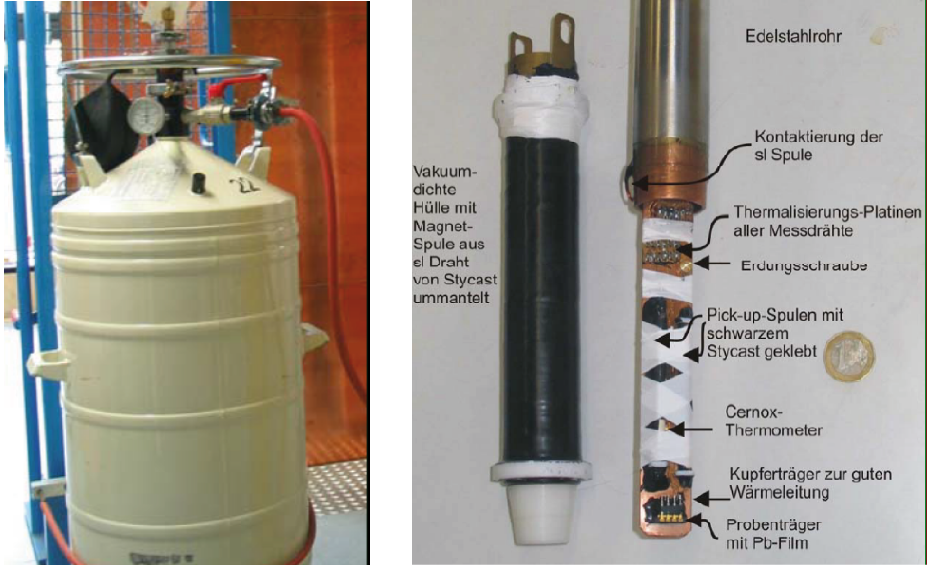
\includegraphics[width=15cm]{tieftemp_aufbau}
		\caption{links: Helium-Kanne. rechts: Versuchsaufbau im Probenkörper, befestigt an einem Edelstahlrohr, welcher in die Helium-Kanne gesenkt wird.}
		\label{tieftemp_aufbau}
	\end{center}
\end{figure}

\subsection{Messungen am Spulenkörper}
Der Strom durch die Magnetspule wurde von 0 bis 4A und wieder zurück auf 0 gesweept. Dabei wurde die induzierte Spannung des Spulenkörpers gegen den Strom durch die Magnetspule aufgetragen. Mit der Gleichung des Magnetfelds einer langen Spule 

\[B=\mu_{0}\dfrac{N}{l}\cdot I \cite{drans}\]
ergibt sich also bei 4A eine maximale Magnetfeldstärke von 0,2T. Die Windungszahl $N$ der Spule betrug $N=6245$, die Länge l der Spule 15,8cm und die magnetische Feldkonstante $\mu_{0}$ beträgt ca. $\SI{1,257e-6}{\newton\per\square\ampere}$.

Eine beispielhafte Messkurve ist in Abb. \ref{4,45} zu sehen. Es handelt sich hierbei um die Messung der Spule bei 4,45K. Die Kurve beginnt im oberen Ast des Graphen bei 0T und bleibt bis zu einer kritischen Magnetfeldstärke von $B_{c}\approx\SI{0,052}{\tesla}$ relativ konstant bei $U_{ind}\approx\SI{0,3}{\milli\volt}$, was durch die Magnetfeldverdrängung eines Supraleiters (Meißner-Effekt) zu erwarten war. Bei Erreichen der kritischen Magnetfeldstärke $B_{c}$ wird der Bleikern der Spule schlagartig normalleitend, wodurch sich eine hohe Flussänderung durch die Spule ergibt, welche zu einem kurzen und hohen Anstieg der induzierten Spannung führt. Danach bleibt die induzierte Spannung bei einem konstanten Wert von ca. 1,1mV. Beim Herunterfahren des Magnetfelds ändert sich mit dem Vorzeichen der Flussänderung auch das Vorzeichen von $U_{ind}$ und die Kurve wird an der x-Achse gespiegelt. Beim kritischen Magnetfeld ist hier nur ein kleiner Peak zu erkennen und anschließend sinkt der Betrag der induzierten Spannung leicht ab. 


\begin{figure}[H]
	\begin{center}
		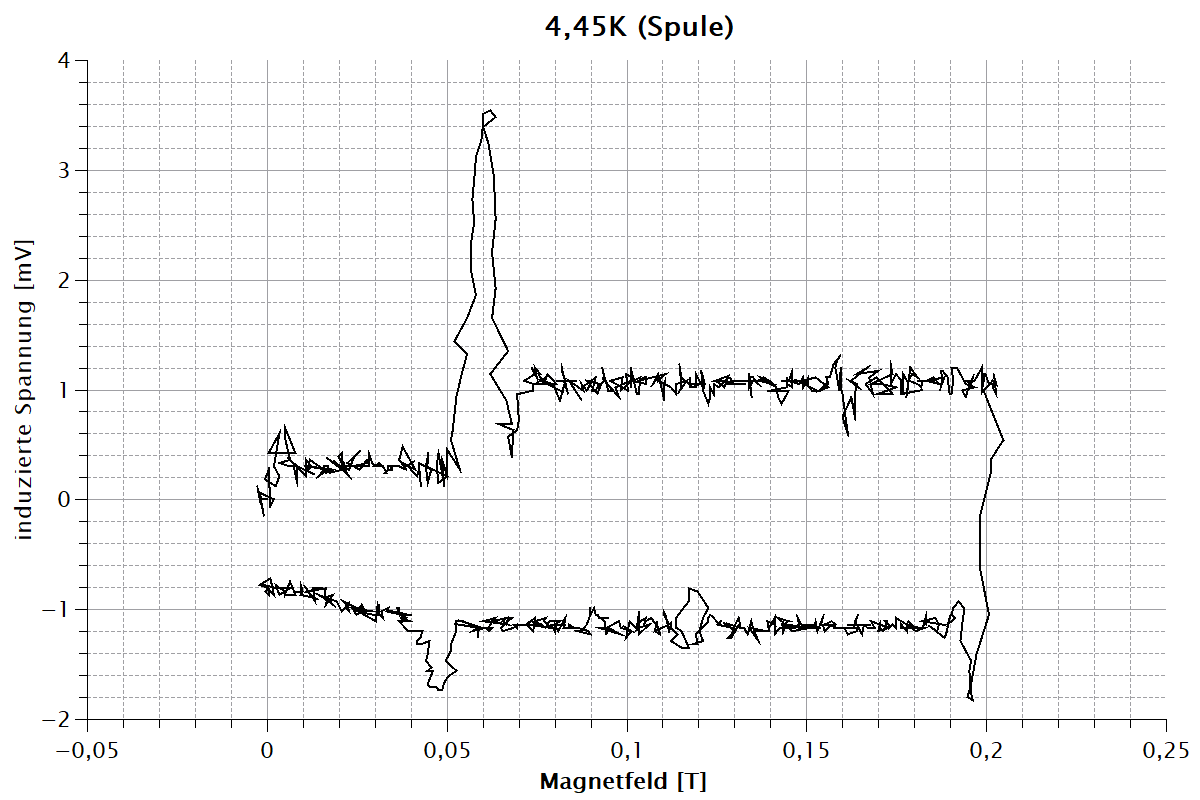
\includegraphics[width=13cm]{4,45.png}
		\caption{Messkurve der Spule bei 4,45K. Gut zu erkennen ist der Peak, eingeleitet durch das Erreichen der kritischen Magnetfeldstärke $B_{c}\approx\SI{0,052}{\tesla}$.}
		\label{4,45}
	\end{center}
\end{figure}

Insgesamt wurden 21 solcher Messkurven bei Temperaturen von 4,45K bis 8,03K aufgenommen. Aus diesen Messreihen wurden dann jeweils die kritischen Magnetfeldstärken $B_{c}$ ermittelt und geplottet, um eine $B_{c} (T)$ Kurve zu erhalten (siehe Abb. \ref{B_c_Spule}). Ab der Messung bei 7,34K setzte der normalleitende Zustand schon ohne Magnetfeld ein, die kritische Temperatur $T_{c}$ war ab hier also überschritten.

Die Kurve wurde mittels qti-plot gemäß der Funktion 

\[B_{c}(T)=B_{c}(0)\cdot\bigg[1-\Big(\dfrac{T}{T_{c}}\Big)^2\bigg] \cite{hunklinger} \] 
gefittet, wobei folgende Werte errechnet wurden:
\begin{itemize}
	\item $B_{c}(0)=\SI{0,0858}{\tesla}$
	\item $T_{c}=\SI{7,31}{K}$ (Literaturwert für Blei: $T_{c}=\SI{7,2}{K}$)
\end{itemize}



\begin{figure}[H]
	\begin{center}
		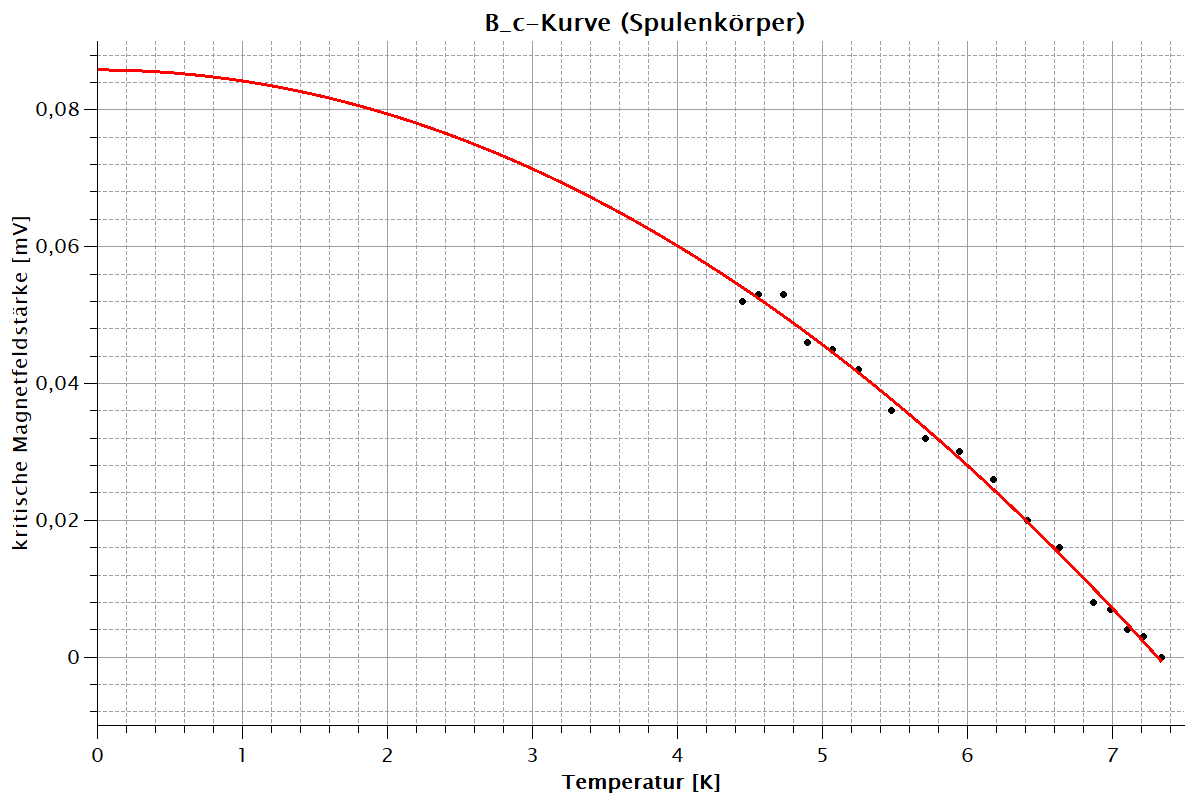
\includegraphics[width=15cm]{B_c_Spule.png}
		\caption{$B_{c}(T)$-Messwerte (schwarz) für den Spulenkörper mit  entsprechendem Fit (rot).}
		\label{B_c_Spule}
	\end{center}
\end{figure}

Zusätzlich sollte noch die magnetische Suszeptibilität $\chi_{s}$ des Bleikerns im supraleitenden Zustand bestimmt werden. Der Index \textit{s} steht hierbei im Folgenden für den supraleitenden Zustand, der Index \textit{n} für den normalleitenden Zustand.
Über die Beziehung 
\[U_{ind}=N_{p}A_{p}\mu_{0}\mu \dfrac{N}{l}\dot{I} \cite{drans}\] 
folgt mit $\mu=1+\chi$:

\[U_{ind}=\dfrac{N_{p}A_{p}\mu_{0}N\dot{I}}{l}(1+\chi)\]
und daraus:

\[\Delta U=U_{ind,n}-U_{ind,s}=\dfrac{N_{p}A_{p}\mu_{0}N\dot{I}}{l}(\chi_{n}-\chi_{s})\]
was sich umformen lässt zu

\[\chi_{s}=-\dfrac{\Delta U l}{N_{p}A_{p}\mu_{0}N\dot{I}}+\chi_{n}\]

hierbei bezeichnet
\begin{itemize}
	\item $\Delta U=U_{ind,n}-U_{ind,s}$ den gemittelten Unterschied der induzierten Spannung zwischen dem supraleitenden und dem normalleitenden Zustand (siehe Abb. \ref{delta_u}), $\Delta U\approx\SI{0,8}{\milli\volt} $
	\item $l$ die Länge der Magnetfeldspule, $l=\SI{15,8}{\centi\meter}$
	\item $N_{p}$ die Windungszahl des Spulenkörpers, $N_{p}=2900$
	\item $A_{p}$ die Querschnittsfläche des Spulenkörpers, $A_{p}=\pi r^2=\pi (\SI{2,1}{\milli\meter})^2=\SI{13,85e-6}{\square\meter}$
	\item $\mu_{0}$ die magnetische Feldkonstante, $\mu_{0}\approx\SI{1,257e-6}{\newton\per\square\ampere}$
	\item $N$ die Windungszahl der Magnetfeldspule, $N=6245$
	\item $\dot{I}$ die zeitliche Ableitung des Stroms durch die Magnetfeldspule, $\dot{I}=\dfrac{\SI{4}{\ampere}}{\SI{8}{\second}}=\SI{0,5}{\ampere\per\second}$
	\item$\chi_{n}\approx\SI{-1,8e-6}{}$
	\end{itemize}

Mit diesen Werten ergibt sich
\[\chi_{s}\approx-0,80\]
Zu erwarten wäre hier ein Wert von exakt -1 gewesen. Mögliche Gründe für die Abweichung sind zum einen die Bestimmung von $\Delta U$ aus den verrauschten Messkurven. Einen großen Beitrag zur Ungenauigkeit des Ergebnisses liefert jedoch auch der Radius des Spulenkörpers: wird für den Radius z.B. $r=\SI{2}{\milli\meter}$ benutzt, was dem Innenradius der Spule entspricht, ergibt sich für die Suszeptibilität ein Wert von $\chi_{s}\approx-0,88$.

\begin{figure}[H]
	\begin{center}
		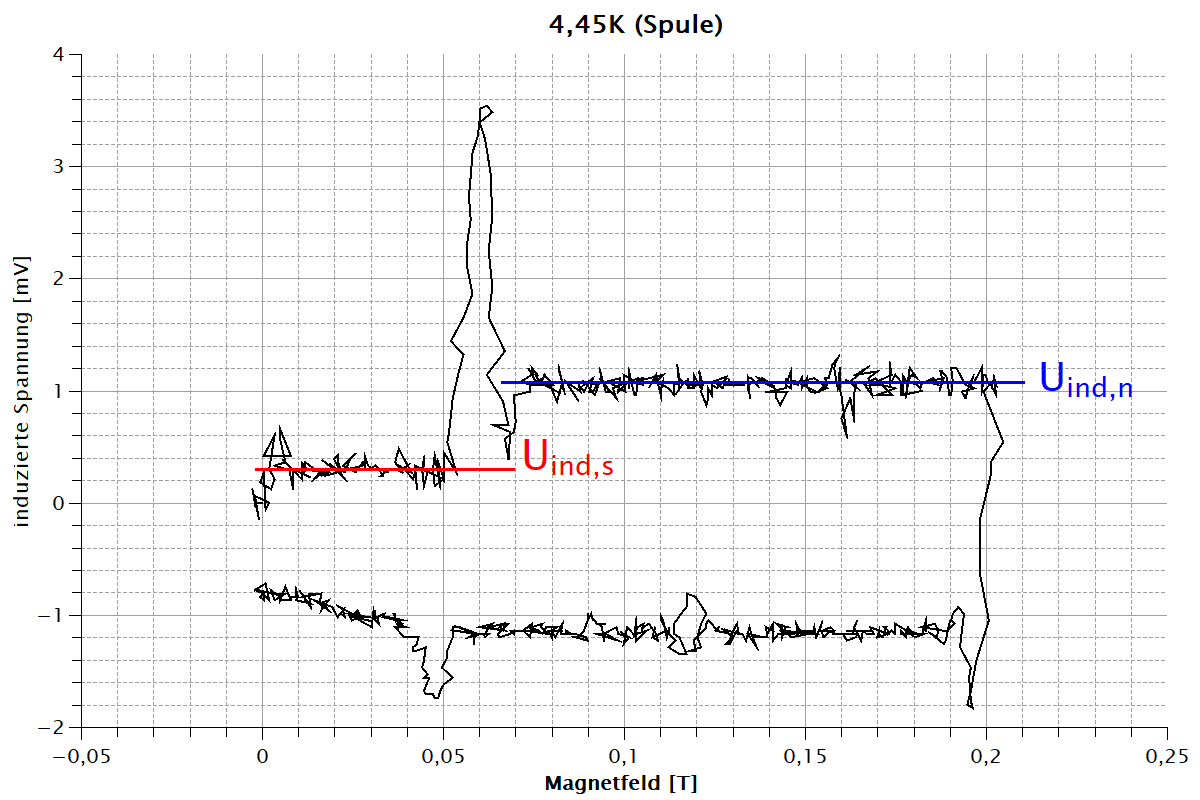
\includegraphics[width=15cm]{delta_u.png}
		\caption{Bestimmung von $\Delta U$ aus den Messkurven. Es wurde hierbei über mehrere Diagramme gemittelt.}
		\label{delta_u}
	\end{center}
\end{figure}

\subsection{Messungen am Niob-Film}

Hier sollten R(B)-Kurven bei verschiedenen Temperaturen (13 Messungen von 8,06K bis 9,19K) aufgenommen werden. Dazu wurde durch den Niob-Film ein konstanter Strom von $\SI{8}{\micro\ampere}$ geschickt und die abfallende Spannung gemessen. Ansonsten war das Verfahren analog zum vorherigen Teil. Die so erhaltenen U(B)-Kurven konnten dann mithilfe der Beziehung $R=U/I$ in R(B)-Kurven umgewandelt werden. Ein beispielhaftes Diagramm ist in Abb. \ref{8,73_film} zu sehen.

Von den jeweiligen R(B)-Kurven wurde jeweils der Widerstand bei $B=\SI{0}{\tesla}$ ermittelt, um eine R(T)-Kurve für das Nullfeld zu ermitteln, woraus sich die Sprungtemperatur zu $T_{c}\approx\SI{9}{\kelvin}$ ermitteln lässt (siehe Abb. \ref{R(T)}). Der Literaturwert hierzu liegt bei $\SI{9,2}{K}$.

 \begin{figure}[H]
 	\begin{center}
 		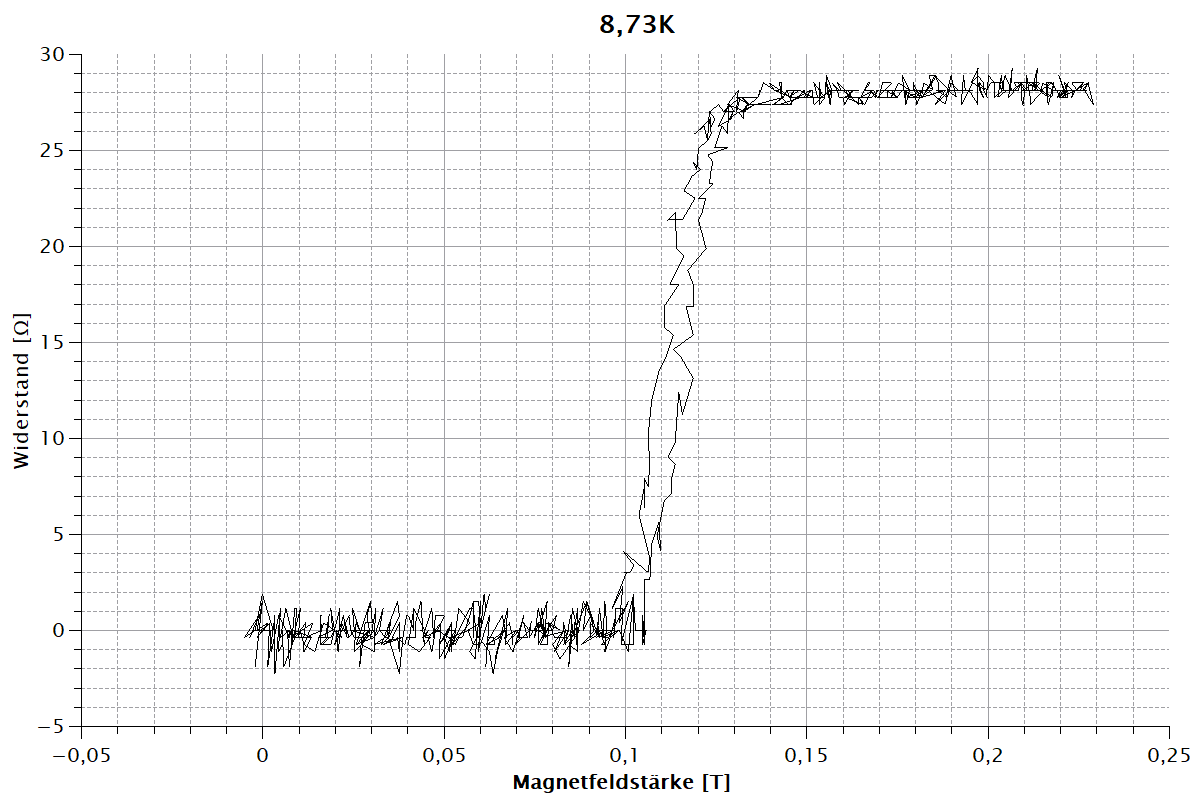
\includegraphics[width=13cm]{8,73_Film.png}
 		\caption{R(B)-Kurve des Niob-Films bei einer Temperatur von 8,73K. Das kritische Magnetfeld liegt hier ca. bei $\SI{0,11}{\tesla}$}
 		\label{8,73_film}
 	\end{center}
 \end{figure}

\begin{figure}[H]
	\begin{center}
		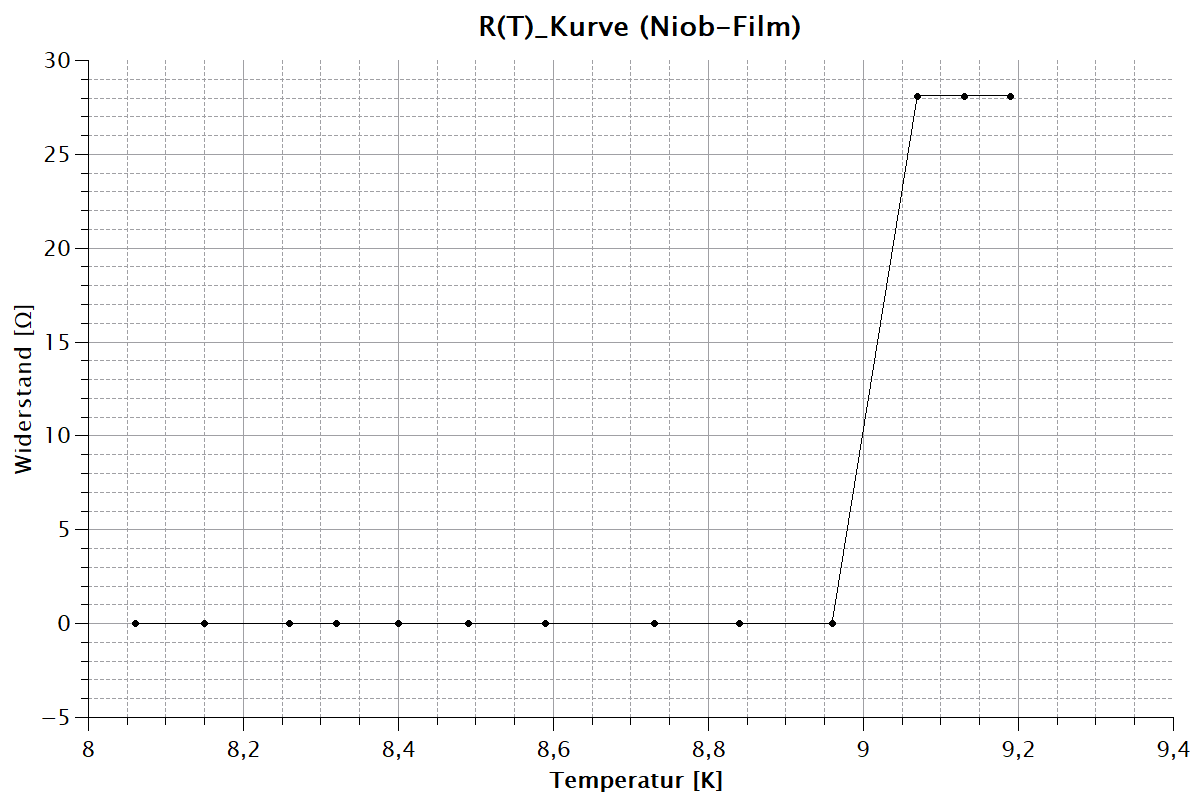
\includegraphics[width=13cm]{R(T).png}
		\caption{R(T)-Kurve des Niob-Films. Die Sprungtemperatur $T_{c}$ liegt ca. bei 9K.}
		\label{R(T)}
	\end{center}
\end{figure}

Zusätzlich sollte hier ebenfalls eine $B_{c}(T)$-Kurve, analog zu Kapitel 3.1.1,  angefertigt werden. Diese ist in Abb. \ref{B_c_film} dargestellt. Die Fitparameter ergaben für die kritische Magnetfeldstärke bei $\SI{0}{\kelvin}$ $B_{c}(0)=\SI{1,82}{\tesla}$ und für die Sprungtemperatur $T_{c}=\SI{8,99}{K}$.

\begin{figure}[H]
	\begin{center}
		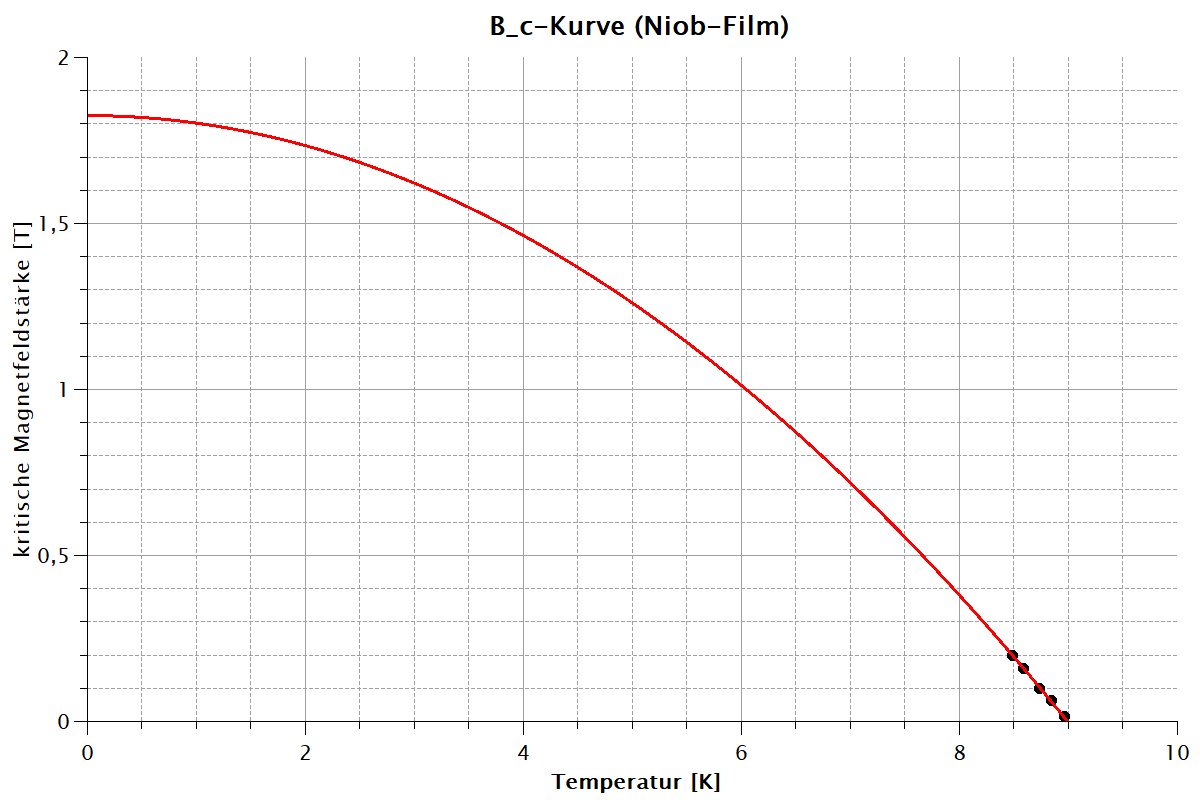
\includegraphics[width=15cm]{B_c_Film.png}
		\caption{Messwerte der kritischen Magnetfeldstärke (schwarz) mit Fit-Kurve (rot). Gut zu erkennen ist $B_{c}(0)=\SI{1,82}{\tesla}$ (Schnittpunkt mit der y-Achse). Die errechnete kritische Temperatur liegt bei $T:{c}=\SI{8,99}{\kelvin}$.}
		\label{B_c_film}
	\end{center}
\end{figure}


\section{Hochtemperatur Supraleitung}
In diesem Versuchsteil sollten die R(T)-Kurven einer YBCO-Tablette für a-b-Leitung, sowie für c-Leitung aufgenommen werden. Dazu wurde der YBCO-Kristall in flüssigen Stickstoff getaucht und somit langsam auf 77K abgekühlt. Die Temperatur des Kyrostaten wurde dabei mit Hilfe eines Thermoelements ermittelt. Zur Bestimmung des Widerstands wurde ein konstanter Strom ($I=1,55$mA) durch den Kristall geleitet und die an der Tablette abfallende Spannung mittels eines Lock-In Verstärkers ermittelt. Dadurch konnte über die Beziehung $R=U/I$ der Widerstand errechnet werden. Kurz nach dem Eintauchen des Kristalls in den flüssigen Stickstoff wurde ein Messprogramm am Computer gestartet, welches im Abstand von einer Sekunde die an der Tablette abfallende Spannung gegen die Thermospannung des Thermoelements auftrug. Der Versuchsaufbau ist in Abb. \ref{hoch_aufbau} dargestellt. 

Dieser Versuchsteil konnte von uns nicht korrekt durchgeführt werden, da sich während der Messung in c-Richtung herausstellte, dass der Probenkörper ein Leck hatte und somit der flüssige Stickstoff direkt mit dem Kristall in Kontakt kommen konnte, was die Messung verfälschte (siehe Abb. \ref{fail}). \textbf{In Rücksprache mit dem Betreuer verwenden wir deshalb für diesen Teil die Messergebnisse einer anderen Praktikumsgruppe.} Leider ist uns deswegen auch die für die Widerstandsbestimmung benötigte konstante Stromstärke nicht bekannt, weswegen wir hierfür unseren Wert ($ I= \SI{1,55}{\milli\ampere}$) verwenden. 
Zur Umrechnung der Thermospannung in Temperatur verwendeten wir die im Anhang der Anleitung gegebene Näherung:
\[T\approx \sqrt{\dfrac{U}{0,0637}+16111} - \SI{49,5}{\kelvin}\]
wobei $U$ die \textbf{Thermospannung in Mikrovolt} bezeichnet. 

\begin{figure}[H]
	\begin{center}
		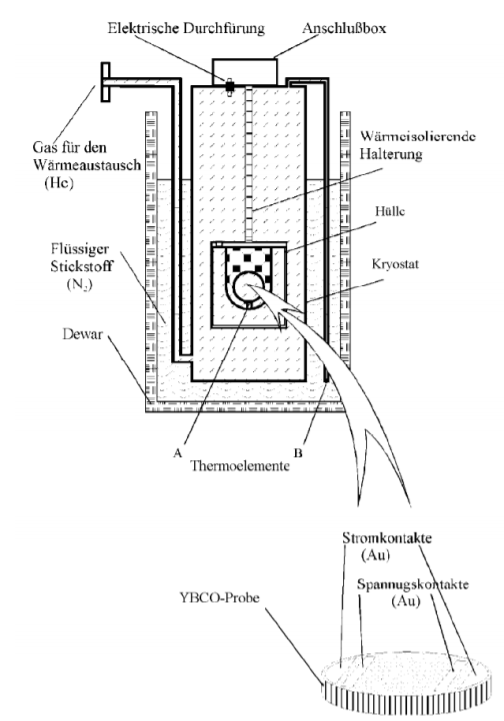
\includegraphics[width=7cm]{hochtemp_aufbau.png}
		\caption{Schematische Darstellung des Versuchsaufbaus zur Hochtemperatur-Supraleitung.}
		\label{hoch_aufbau}
	\end{center}
\end{figure}

\begin{figure}[H]
	\begin{center}
		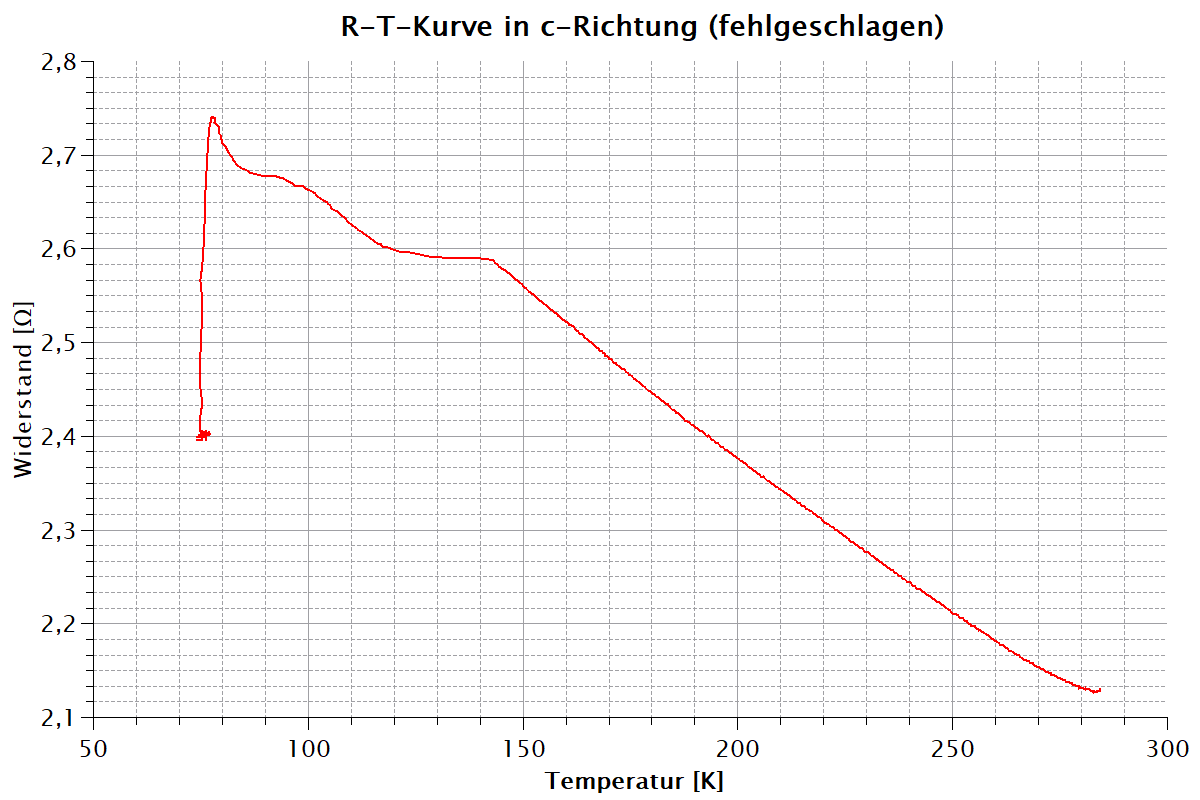
\includegraphics[width=17cm]{fail.png}
		\caption{Fehlgeschlagene Messung in c-Richtung. Auffällig ist der unregelmäßige Verlauf der Kurve unterhalb von 150 K. Außerdem liegt hier die gemessene Sprungtemperatur bei ca. 78 K, was weit unter dem Literaturwert ($T_{c}=\SI{92}{K}$) liegt. }
		\label{fail}
	\end{center}
\end{figure}


\subsection{a-b-Richtung} %Quellenangabe
Die a-b-Ebene bezeichnet beim YBCO-Kristall die Ebene, in der die $CuO_{2}$-Schichten liegen, welche zum einen für die Ausbildung der Supraleitung verantwortlich sind und zum anderen auch im normalleitenden Zustand die höchste Leitfähigkeit besitzen. Deshalb ist hier oberhalb der Sprungtemperatur ein geringerer Widerstand zu erwarten als bei der Messung senkrecht zu den $CuO_{2}$-Schichten, also in c-Richtung.

Beim Verlauf der R(T)-Kurve (siehe Abb. \ref{ab})  fällt auf, dass der Widerstand zunächst mit sinkender Temperatur steigt, wodurch schon erkannt werden kann, dass es sich beim YBCO-Kristall um keinen metallischen Leiter handelt, da hier ein gegenteiliges Verhalten zu erwarten wäre.

Die Sprungtemperatur $T_{c}$ konnten wir zu $T_{c}\approx\SI{92}{\kelvin}$ bestimmen, was dem Literaturwert entspricht. \cite{hunklinger}

Bei beiden Messungen tritt ein Offset in y-Richtung auf, d.h. auch unterhalb der Sprungtemperatur fällt der gemessene Widerstand des Kristalls nicht auf exakt Null. Dieser Offset ist durch die Übergangswiderstände der Messkontakte zu erklären, welche durch den Übergang von Metall (vergoldete Messkontakte) auf Keramikmaterial (YBCO-Tablette) zustande kommen. Der Offset liegt bei der Messung in a-b-Richtung bei ca. $\SI{1}{\ohm}$ in c-Richtung bei ca. $\SI{1,8}{\ohm}$.

\begin{figure}[H]
	\begin{center}
		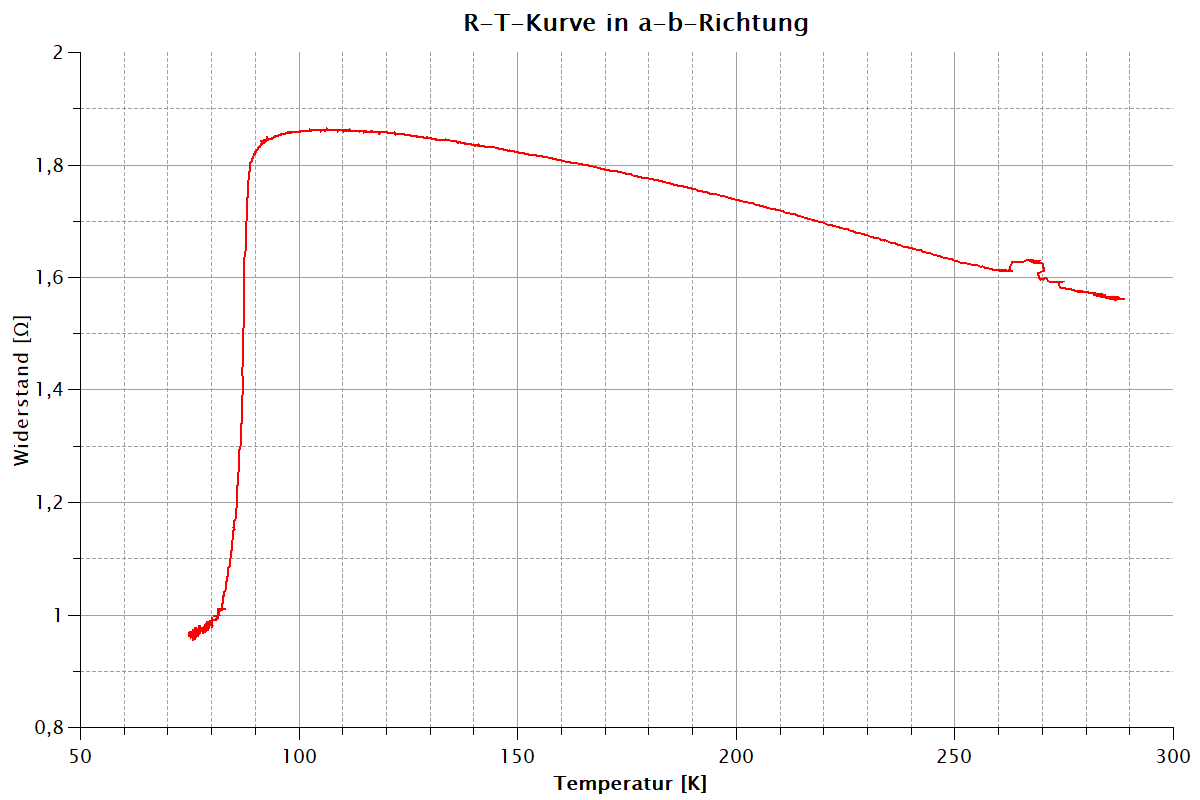
\includegraphics[width=15cm]{a-b.png}
		\caption{R(T)-Kurve der Messung in a-b-Richtung. Der steile Abfall des Widerstandes ist deutlich zu sehen, bei einer Sprungtemperatur von ca. $\SI{92}{\kelvin}$. Der Offset liegt bei ca. $\SI{1}{\ohm}$.}
		\label{ab}
	\end{center}
\end{figure}

\subsection{c-Richtung}
Die Messung in c-Richtung ergab eine relativ ähnliche R(T)-Kurve wie in a-b-Richtung (siehe Abb. \ref{c}), jedoch - wie zu erwarten - mit etwas höheren Widerständen in der normalleitenden Phase. Die Sprungtemperatur konnten wir zu $T_{c}\approx\SI{93}{\kelvin}$ bestimmen.

\begin{figure}[H]
	\begin{center}
		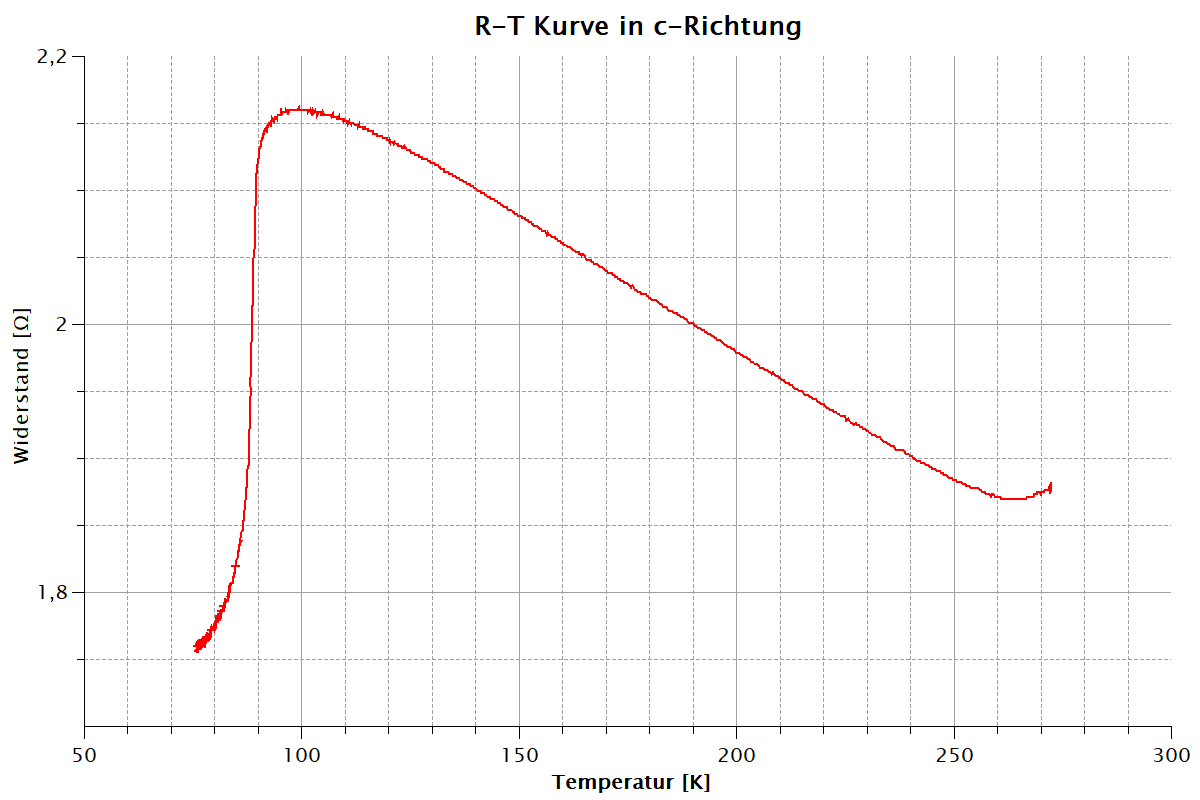
\includegraphics[width=15cm]{c.png}
		\caption{R(T)-Kurve in c-Richtung. Im Vergleich zur a-b-Richtung ist die normalleitende Phase um ca. $\SI{0,3}{\ohm}$ nach oben verschoben (zu beachten ist die unterschiedliche Skalierung der y-Achsen!). Die Sprungtemperatur liegt bei ca. 93K, der Offset bei ca. $\SI{1,8}{\ohm}$. }
		\label{c}
	\end{center}
\end{figure} 
 
 
\section{Levitation}
Im letzten Versuchsabschnitt wurde die Levitation eines Supraleiters untersucht. Dazu wurde eine YBCO-Tablette und ein kleiner Permanentmagnet verwendet.

Zuerst wurde die Tablette in einer Schale mit flüssigem Stickstoff unter die Sprungtemperatur abgekühlt. Mit einer Pinzette näherten wir nun den Magneten an die Tablette an und stellten eine deutliche abstoßende Kraft fest. Erklären lässt sich dies durch die Magnetfeldverdrängung eines Supraleiters. Die YBCO-Tablette ist im supraleitenden Zustand perfekt diamagnetisch, das heißt sie baut ein gleich großes Gegenfeld zum Magnetfeld des Permanentmagneten auf, was dann durch die abstoßende Kraft bemerkbar wird. Wir konnten so jedoch keinen Zustand herstellen, in dem der Magnet über der Tablette schwebt. Um dies zu erreichen, legten wir die Tablette in die leere Schale, positionierten darauf ein kleines Stück Styropor als Abstandhalter und legten darauf den Magneten. Anschließend wurde die Tablette wieder mit flüssigem Stickstoff abgekühlt. Nach Entfernen des Abstandhalters schwebte der Magnet über dem YBCO Kristall (siehe Abb. \ref{schwebt}). Der Magnet konnte sogar für wenige Sekunden mit einer Pinzette angehoben und gedreht werden, während die Tablette weiterhin unter dem Magneten schwebte (siehe Abb. \ref{levitation}). Erklären lässt sich dieses Phänomen dadurch, dass das Magnetfeld des Magneten die YBCO-Tablette im normalleitenden Zustand durchdringen kann. Beim Abkühlen unter die Sprungtemperatur bilden sich nun magnetische Flussschläuche im Supraleiter aus, welche von ringförmigen Abschirmströmen umgeben werden. Der Supraleiter als idealer Diamagnet wirkt nun jeder Änderung des Magnetfelds entgegen, wodurch der energetisch günstige Zustand somit dann erreicht ist, wenn sich die relative Position der Tablette zum Magneten nicht ändert. Wird der Magnet also angehoben, folgt die Tablette in konstantem Abstand. \cite{hunklinger}

\begin{figure}[H]
	\begin{center}
		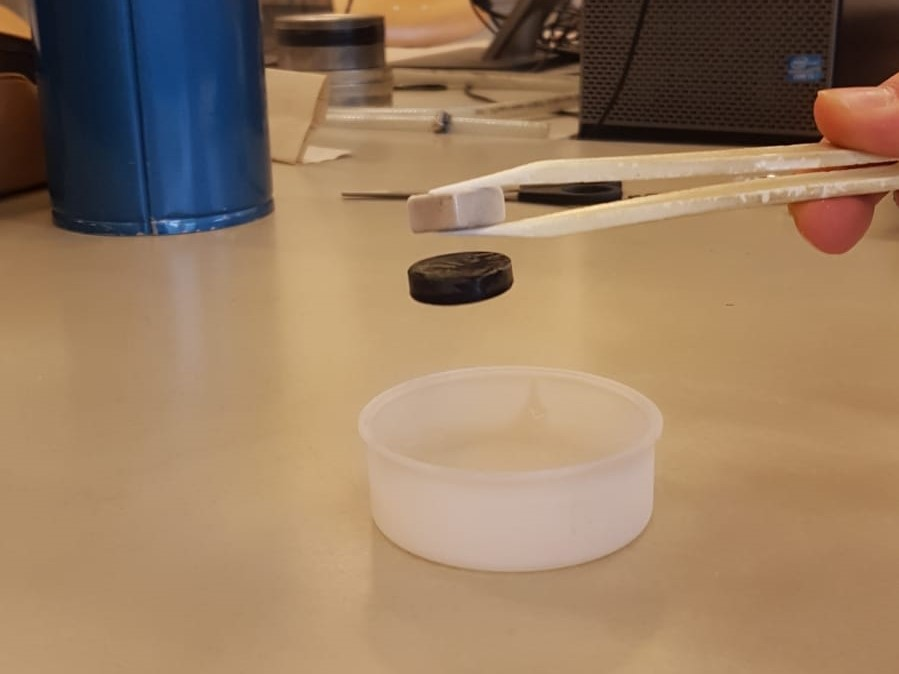
\includegraphics[width=12cm]{levitation}
		\caption{Die YBCO-Tablette schwebt unter dem Permanentmagneten. Unterhalb ist die Schale mit flüssigem Stickstoff zu sehen.}
		\label{levitation}
	\end{center}
\end{figure}

\begin{figure}[H]
	\begin{center}
		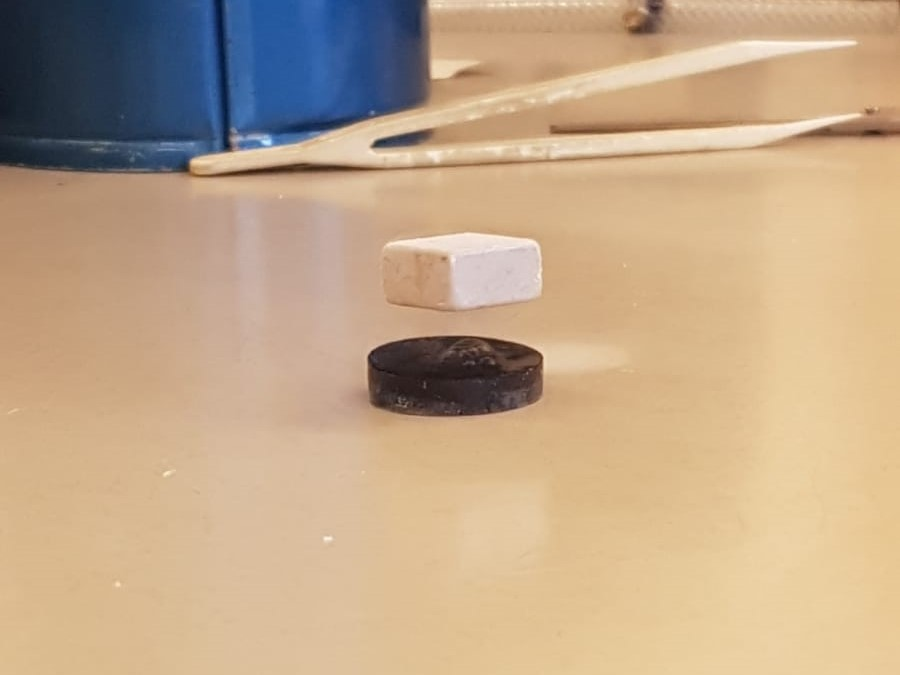
\includegraphics[width=12cm]{schwebt}
		\caption{Der Magnet schwebt über der YBCO-Tablette. Außerhalb vom flüssigen Stickstoff ist dieser Zustand nur wenige Sekunden stabil, bis der Supraleiter sich über seine Sprungtemperatur aufgewärmt hat. Auf der Tablette sind Blasen des siedenden Stickstoffs zu erkennen.}
		\label{schwebt}
	\end{center}
\end{figure}


\chapter{Anhang}
\section{Messkurven zum Tieftemperaturteil (Spulenkörper)}
\begin{figure}[H]
	\begin{center}
		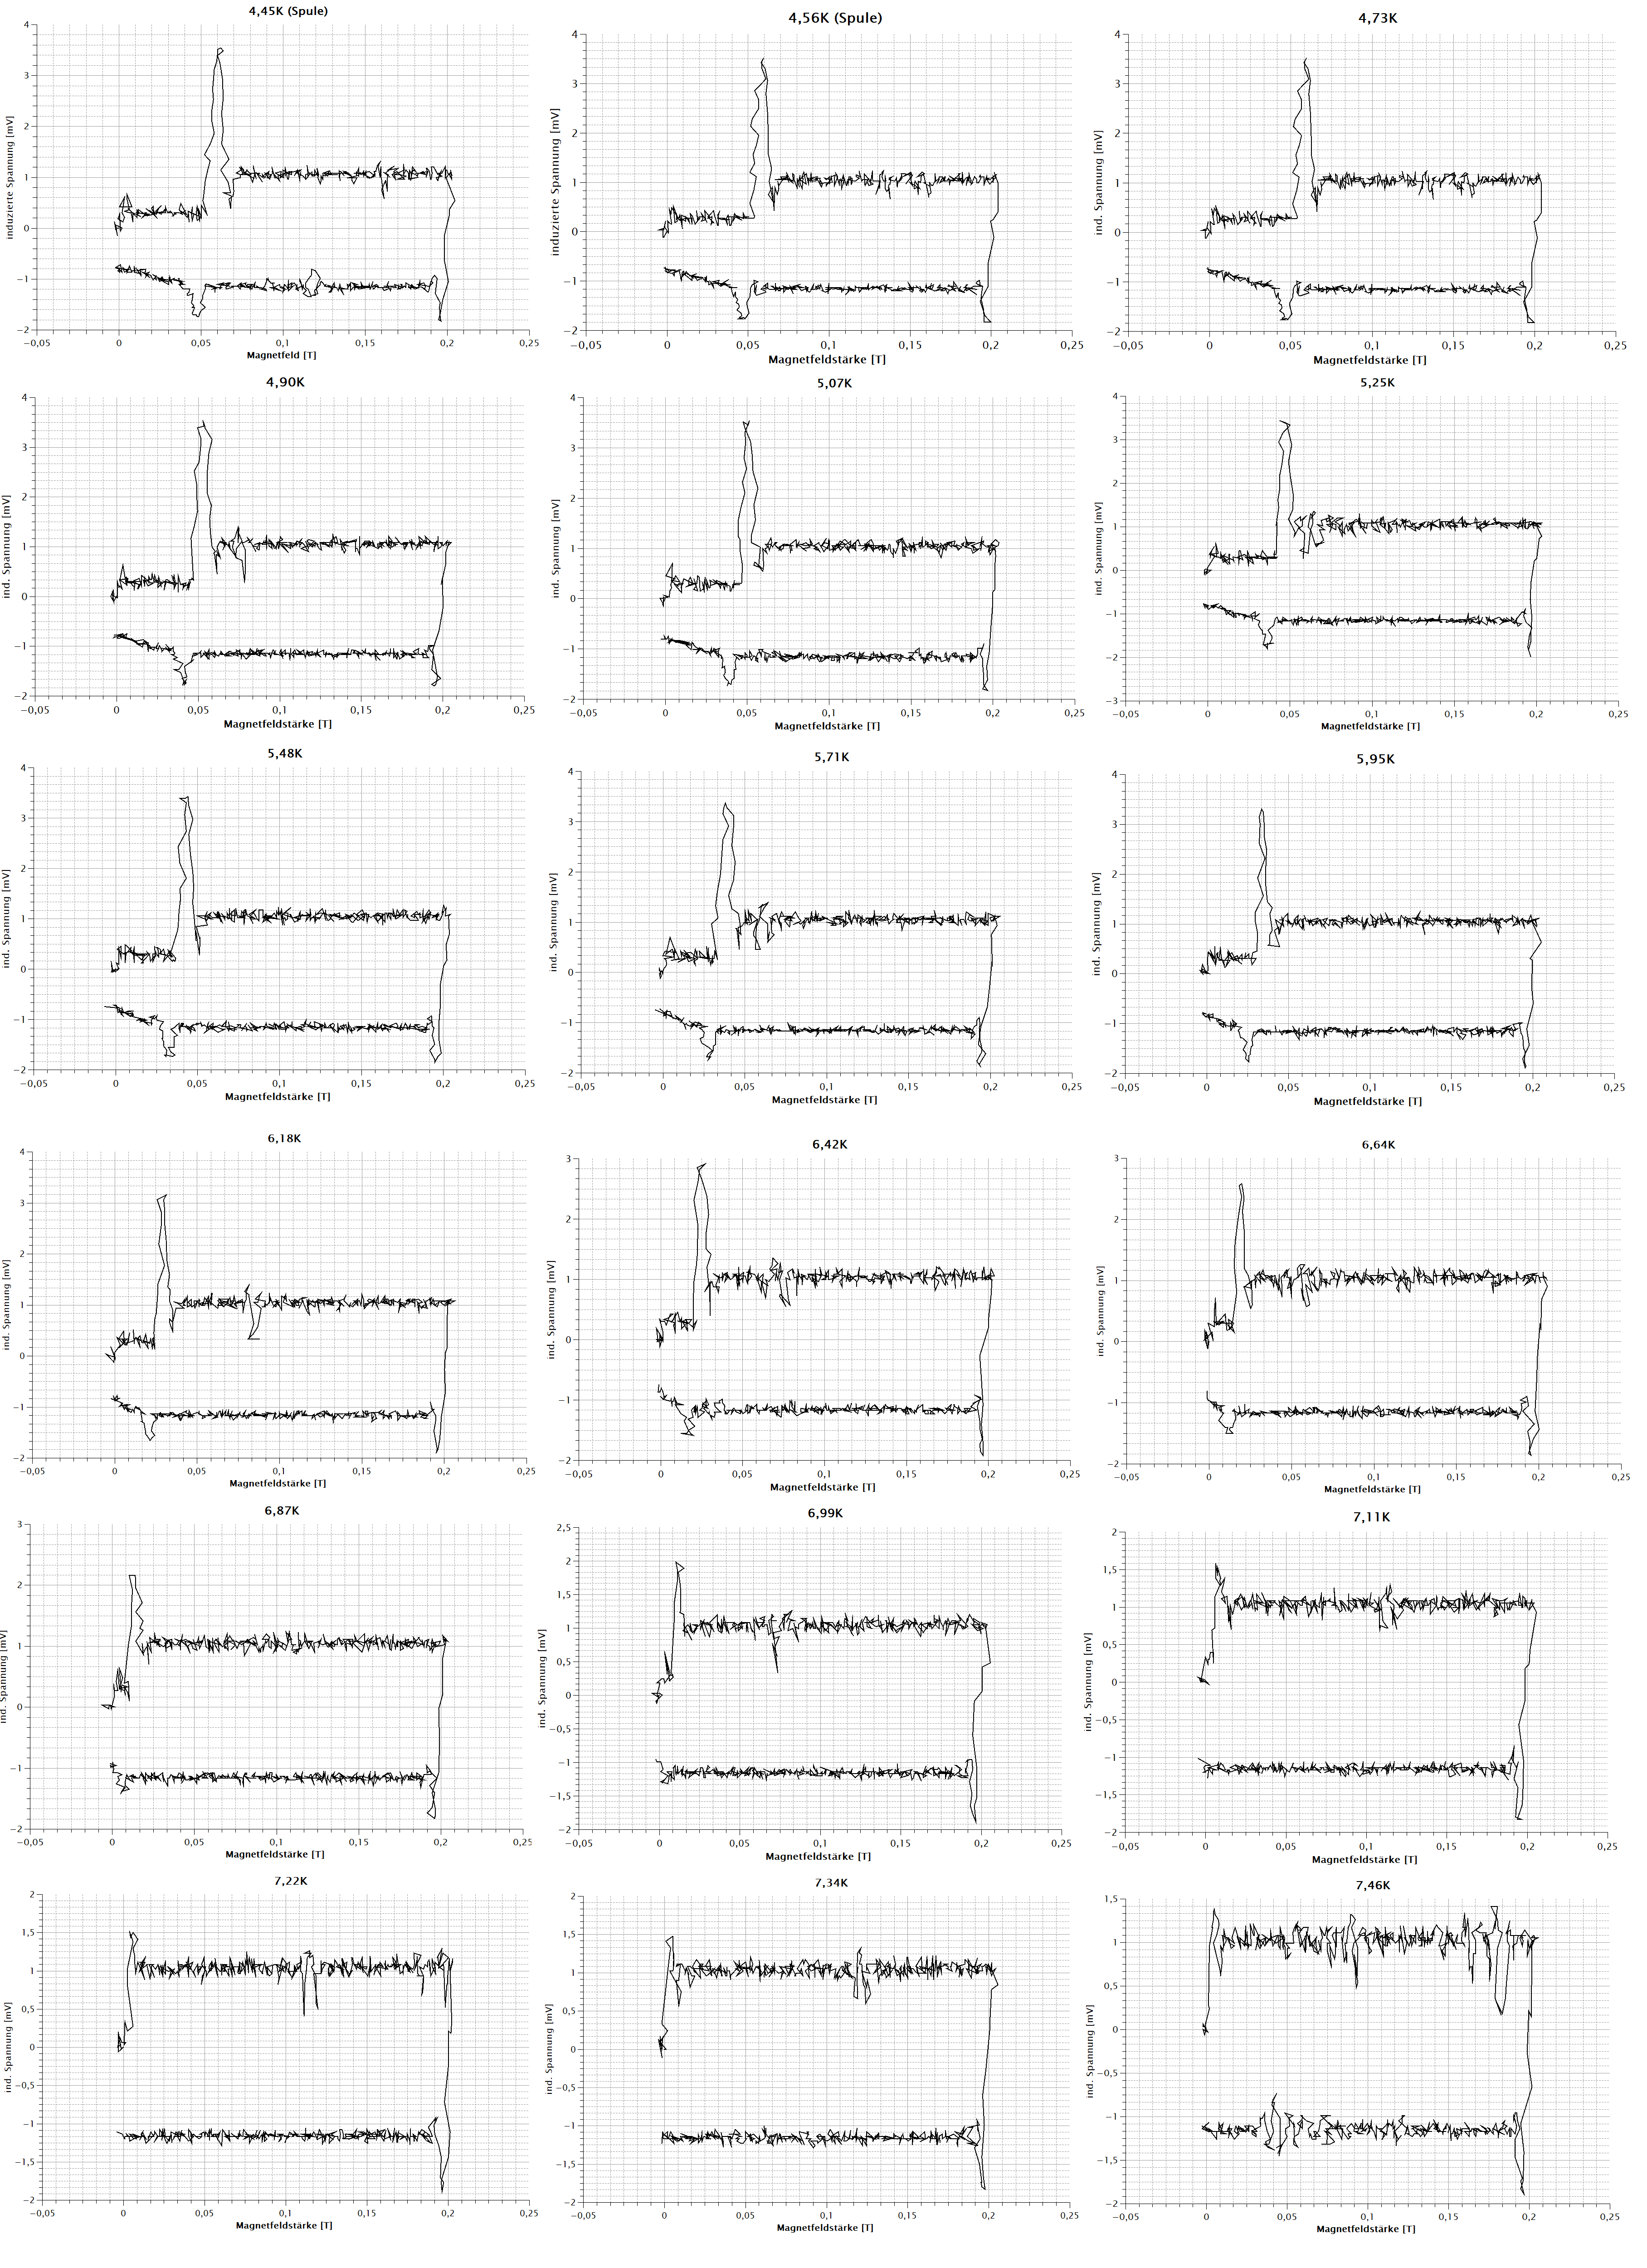
\includegraphics[width=12cm]{graphen_spule.png}
	\end{center}
\end{figure}

\section{Messkurven zum Tieftemperaturteil (Niob-Film)}
\begin{figure}[H]
	\begin{center}
		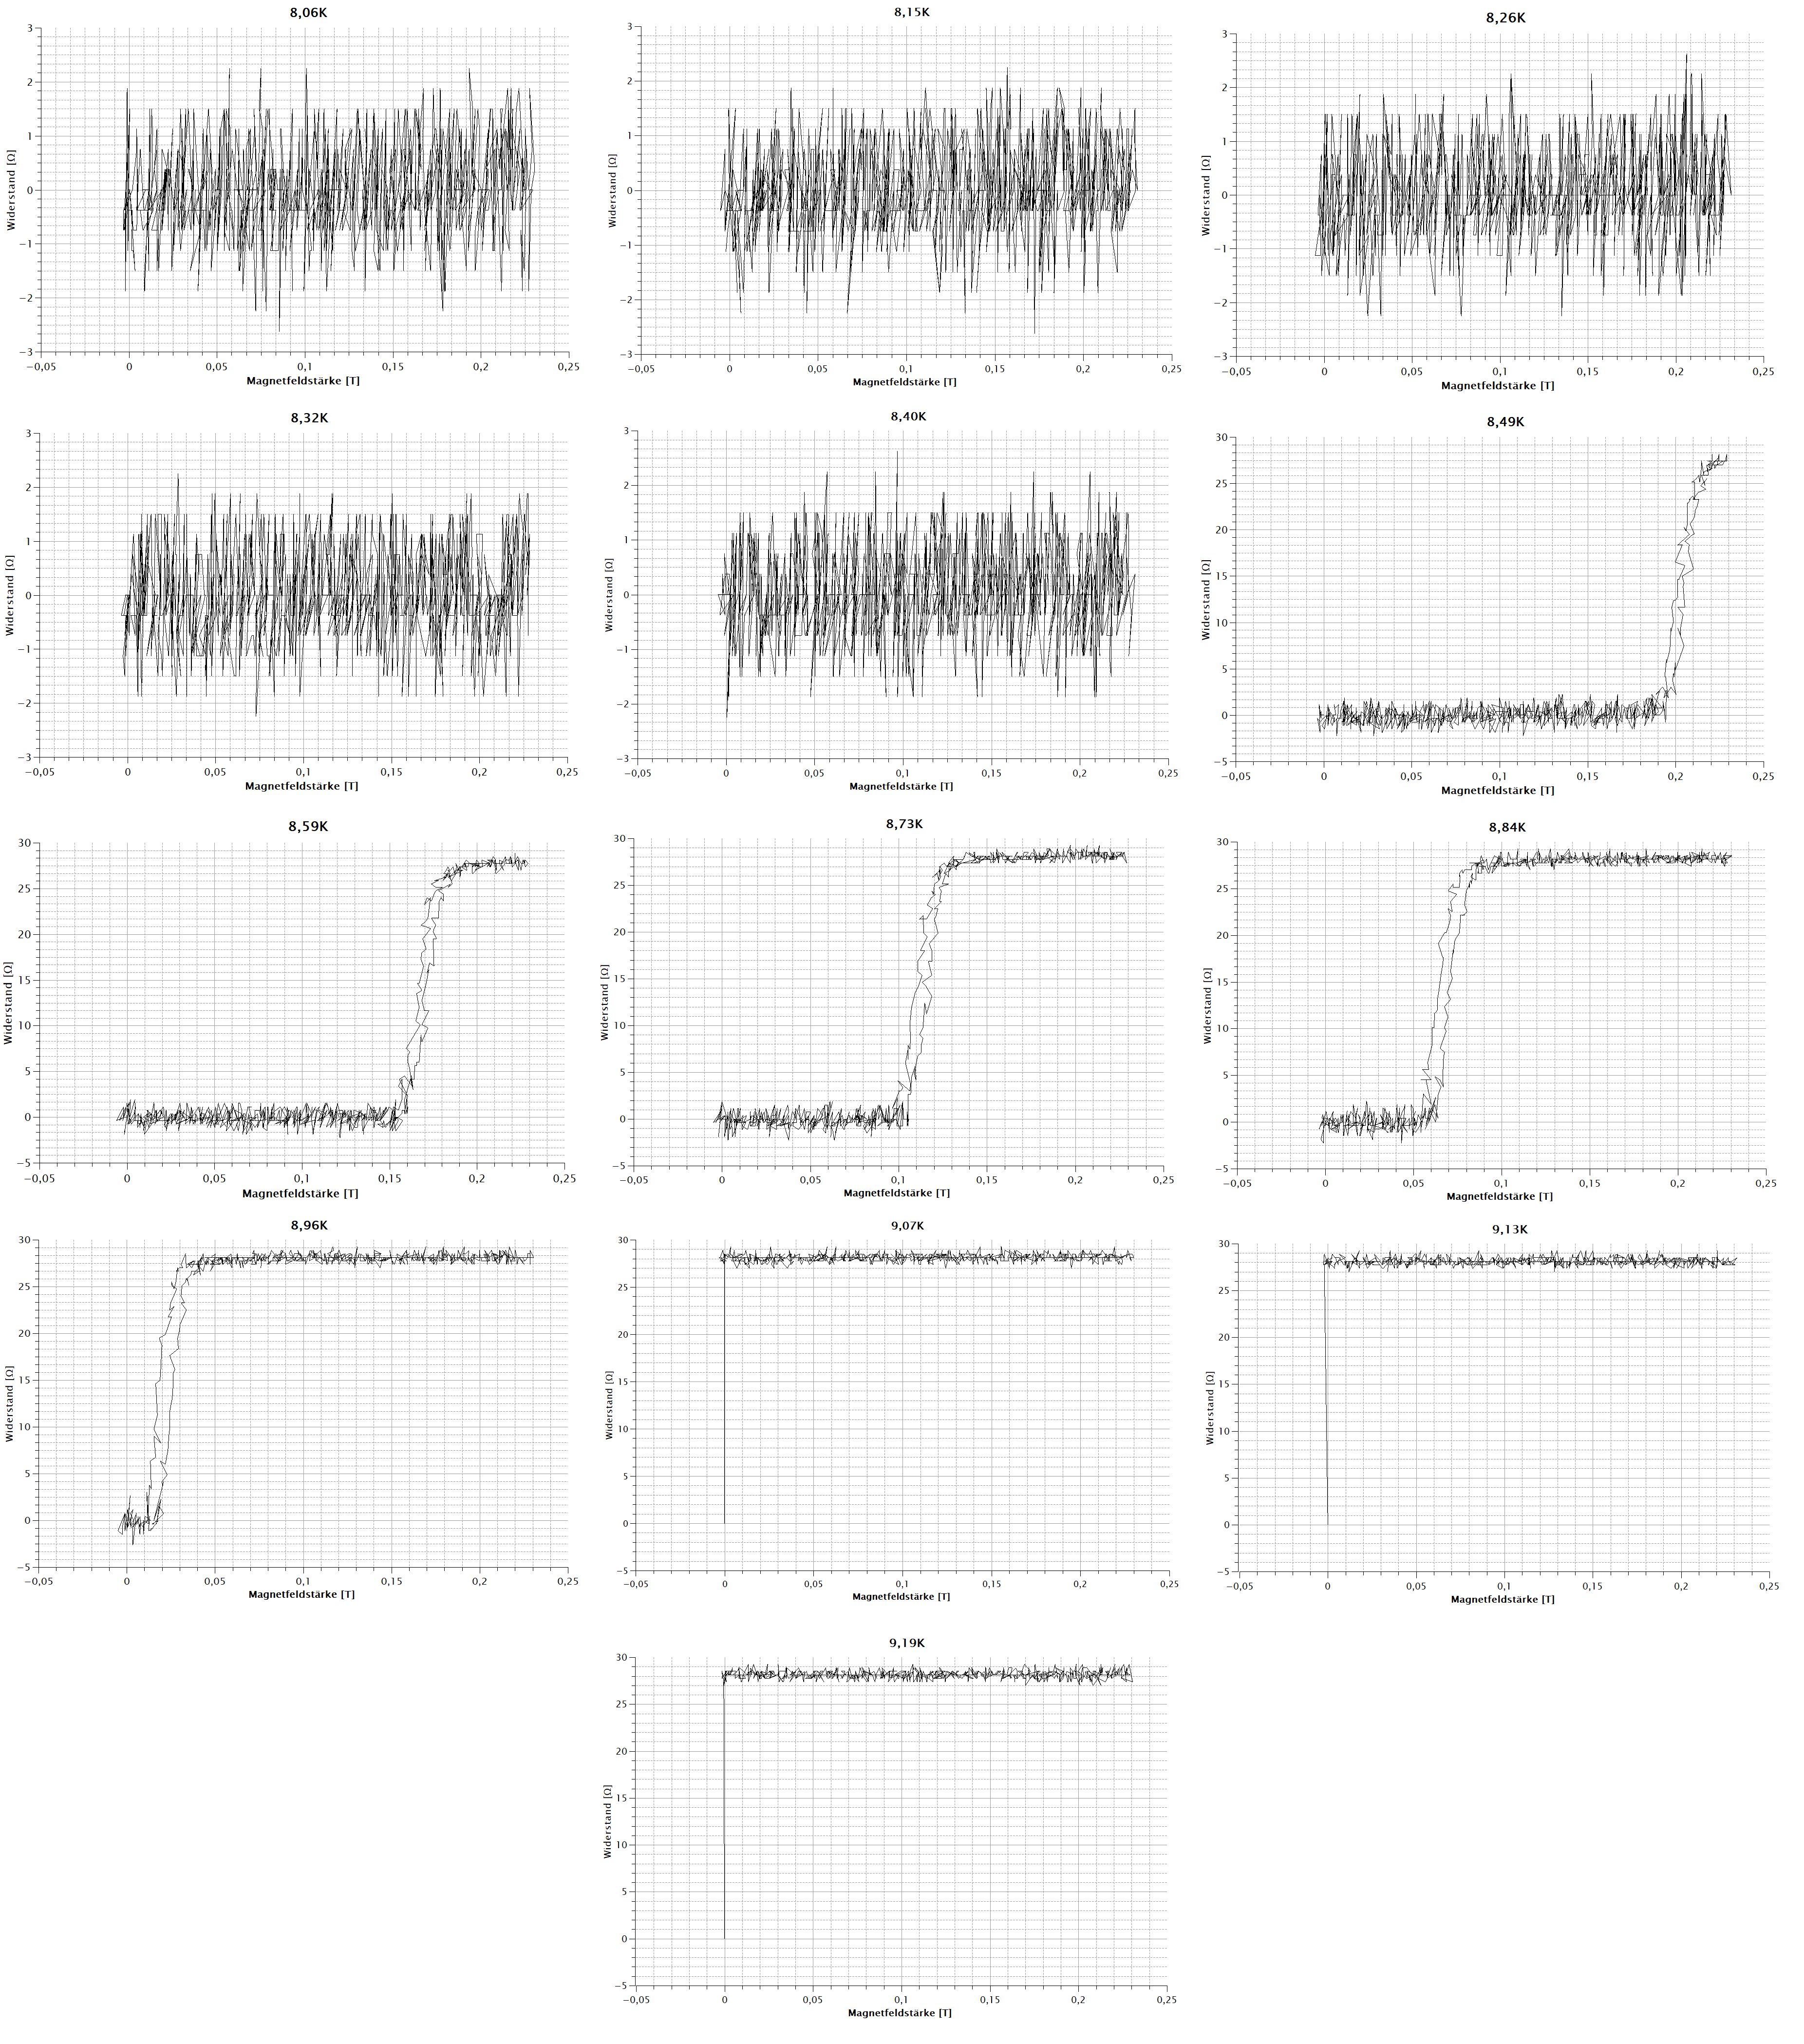
\includegraphics[width=15cm]{graphen_niob}
	\end{center}
\end{figure}
